% !TeX root = ../../../Main.tex
\chapter{Conference Paper}

Give a full bibliographic reference including status of the submission (submitted/accepted/to be presented/published) and describe, very briefly, how the paper addresses the problem the thesis deals with.

\cleardoublepage

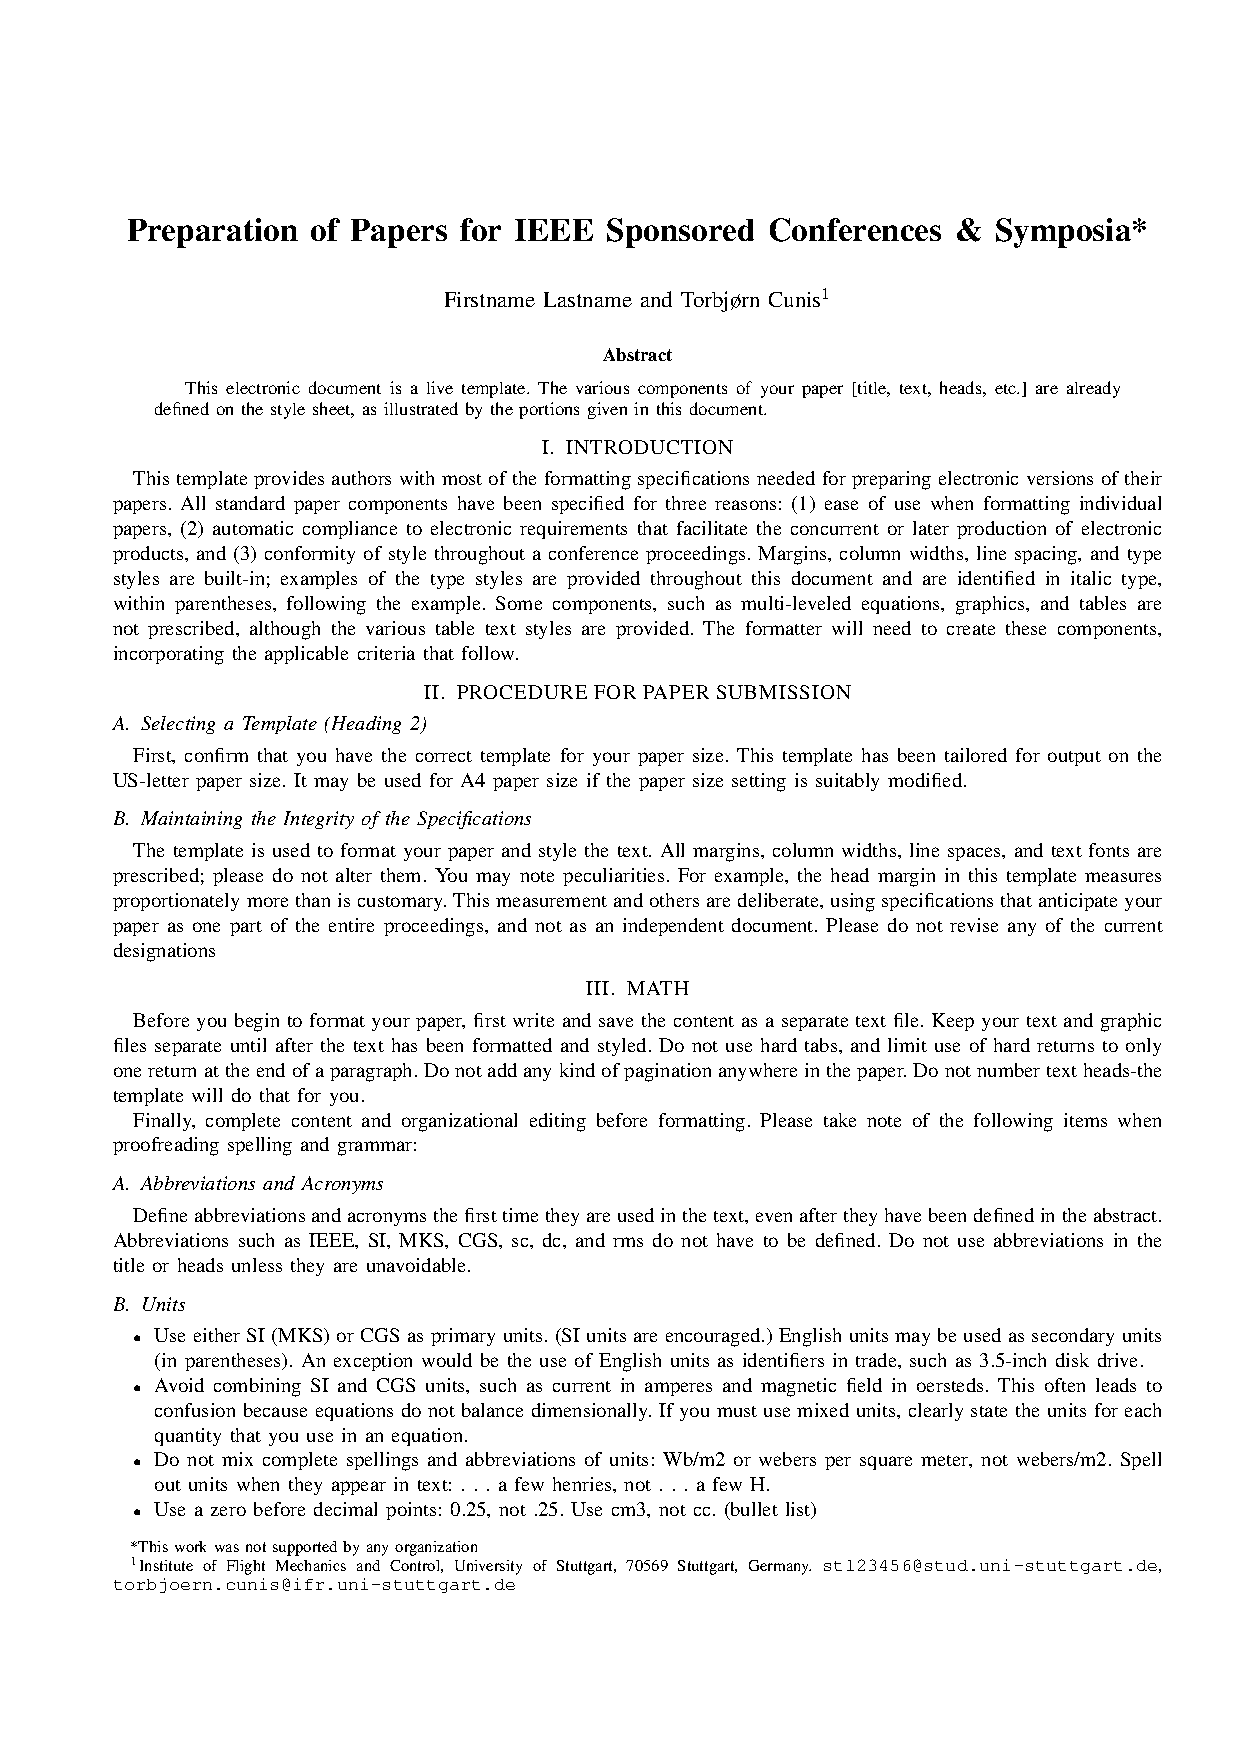
\includepdf[pages=-,
addtotoc={%add paper sections to toc
%syntax: page,level,depth,title,label,
1,section,1,Introduction,sec:paper:introduction,
1,section,1,Procedure for Paper Submission,sec:paper:procedure,
1,subsection,2,Selecting a Template,sec:paper:procedure-selecting,
1,subsection,2,Maintaining the Integrity of the Specifications,sec:paper:procedure-maintaining,
1,section,1,Math,sec:paper:math,
1,subsection,2,Abbreviations and Acronyms,sec:paper:math-acronyms,
1,subsection,2,Units,sec:paper:math-units,
2,subsection,2,Equations,sec:paper:math-equations,
2,subsection,2,Some Common Mistakes,sec:paper:math-mistakes,
2,section,1,Using the Template,sec:paper:usage,
2,subsection,2,{Headings, etc},sec:paper:usage-headings,
2,subsection,2,Figures and Tables,sec:paper:usage-figures,
2,section,1,Conclusions,sec:paper:conclusions,
2,section,1,Appendix,sec:paper:appendix
},
addtolist={%add paper figures and tables to lof/lot
%syntax: page,figure|table,caption,label,
3,table,An example of a table,tab:paper:example,
3,figure,Inductance of oscillation winding on amorphous magnetic core versus DC bias magnetic field,fig:paper:inductance
},
]{./src/parts/mainmatter/paper/root}

% this command parses the paper aux file for citation commands
\externalbibdocument{./src/parts/mainmatter/paper/root}
